\section{Constraints}
Es existieren drei verschiedene Constraints, welche sequentiell in der TCL Console verarbeitet werden.
\begin{itemize}[nosep]
	\item Physical Constraints (I/O placement)
	\item Timing Constraints (Clock definitions)
	\item Configuration Constraints (configuration, bitstream generation)
\end{itemize}

\subsection{XDC Format}
Constraints können in einem XDC File oder direkt in VHDL durch ein Attribut gesetzt werden.
\begin{lstlisting}
-- VHDL signal clk\_100MHz zu Pin Y9
set_property PACKAGE_PIN Y9 [get_ports clk_100MHz]
set_property IOSTANDARD LVCMOS33 [get_ports clk_100MHz]

-- Pull up for resetn signal
set_property PULLTYPE PULLUP [get_ports resetn]
\end{lstlisting}
\vspace{-20pt}

Vivado IO Planner
\begin{center}
	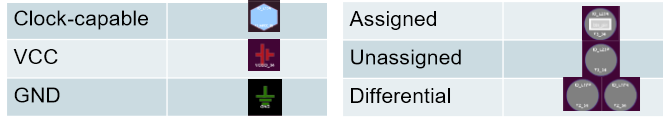
\includegraphics[width=0.8\columnwidth]{Images/ioplanner}
\end{center}

\subsection{Timing}
\begin{itemize}[nosep]
\item \textbf{Clock Distribution} delay $t_{di}$, clock latency: Zeitverzögerung gemessen vom Auftreten der Taktflanke an der Taktquelle bis zum Zustandsübergang am Ziel (Endpunkt)
\item \textbf{Clock Skew} $t_{sk}$: Ungenauigkeit der gleichen Taktflanke, die an verschiedenen Stellen im Taktbereich.
\item \textbf{Clock Jitter} $t_jt$: Variabilität der aufeinanderfolgenden Taktflanken, die an der gleichen Stelle ankommen.
\item \textbf{Slack}: Differenz zwischen benötigter Zeit und Ankunftszeit, auch als Marge bekannt. Negativer Slack $\Rightarrow$ Zeitproblem
\end{itemize}
\begin{center}
	\includegraphics[width=\columnwidth]{Images/slack}
\end{center}

\subsection{Clock}
Alle Clocks sind immer in Nanosek. zu definieren.

\textbf{Beispiel}:
\begin{center}
	\includegraphics[width=\columnwidth]{Images/clock}
\end{center}

\begin{lstlisting}
-- Clock 100MHz mit 50% Duty Cycle
create_clock -name SysClock -period 10 -waveform {0.000 5.000} [get_ports clk]
set_output_delay -clock SysClock -max 1  [get_ports Dout]
set_output_delay -clock SysClock -min -0.5  [get_ports Dout]
-- latency for external devices
set_clock_latency -source 14 [get_clocks SysClock]
-- jitter definition
set_input_jitter SysClock 0.3
-- Path intentionally not meeting timing requirements
set_false_path -from <source> -to <destination>
\end{lstlisting}


\subsection{External Components}
\begin{align*}
	t_{input\_delay} &= t_{c\_ext} + t_{pcq\_FF1} + t_{d\_board1} - t_{c\_b1} \\
	t_{output\_delay} &= t_{pcbq\_FF3} + t_{d\_out} \\
	t_{delay\_on\_FR4\_PCB} &\approx 0.01 \unit{ns/mm}
\end{align*}
	
\begin{center}
	\includegraphics[width=\columnwidth]{Images/clock1}
\end{center}
